% =====================================================================
% Lab 04 --- Secao 3: derivadas de estabilidade
% Incluido por main.tex. Tabelas em tex_s3/ e figuras em resultados_s3/.
% =====================================================================
% gerado por s3_estabilidade.py
\newcommand{\esAlpha}{0.036}
\newcommand{\esAlphaW}{1.898}
\newcommand{\esCD0Fit}{0.02010}
\newcommand{\esCD0FitW}{0.01569}
\newcommand{\esCDaFit}{0.18763}
\newcommand{\esCDaFitW}{0.11440}
\newcommand{\esCDaaFit}{1.48578}
\newcommand{\esCDaaFitW}{1.42705}
\newcommand{\esCDd4}{-0.0034}
\newcommand{\esCDd4W}{0.0181}
\newcommand{\esCDg1}{0.0169}
\newcommand{\esCDg1W}{0.0351}
\newcommand{\esCDproj}{0.02023}
\newcommand{\esCDprojW}{0.02102}
\newcommand{\esCDq}{0.741}
\newcommand{\esCDqW}{0.637}
\newcommand{\esCDref}{0.02033}
\newcommand{\esCDrefW}{0.01553}
\newcommand{\esCL}{0.4702}
\newcommand{\esCL0}{0.48779}
\newcommand{\esCL0w}{0.24275}
\newcommand{\esCLa}{6.759}
\newcommand{\esCLaW}{6.733}
\newcommand{\esCLd4}{0.4027}
\newcommand{\esCLd4W}{0.4005}
\newcommand{\esCLg1}{0.6415}
\newcommand{\esCLg1W}{0.6401}
\newcommand{\esCLq}{7.718}
\newcommand{\esCLqW}{7.552}
\newcommand{\esCM0}{-0.10560}
\newcommand{\esCM0w}{0.02450}
\newcommand{\esCYb}{0.563}
\newcommand{\esCYbW}{0.557}
\newcommand{\esCYd5}{-0.1591}
\newcommand{\esCYd5W}{-0.1585}
\newcommand{\esCYp}{-0.022}
\newcommand{\esCYpW}{-0.040}
\newcommand{\esCYr}{0.170}
\newcommand{\esCYrW}{0.184}
\newcommand{\esClb}{-0.199}
\newcommand{\esClbW}{-0.159}
\newcommand{\esCld3}{-0.1878}
\newcommand{\esCld3W}{-0.1882}
\newcommand{\esCld5}{0.0186}
\newcommand{\esCld5W}{0.0184}
\newcommand{\esClp}{-0.553}
\newcommand{\esClpW}{-0.557}
\newcommand{\esClr}{0.176}
\newcommand{\esClrW}{0.102}
\newcommand{\esCma}{-0.215}
\newcommand{\esCmaW}{-0.180}
\newcommand{\esCmd4}{-2.0074}
\newcommand{\esCmd4W}{-1.9929}
\newcommand{\esCmg1}{-3.0934}
\newcommand{\esCmg1W}{-3.0916}
\newcommand{\esCmq}{-40.64}
\newcommand{\esCmqW}{-40.36}
\newcommand{\esCnb}{-0.133}
\newcommand{\esCnbW}{-0.128}
\newcommand{\esCnd3}{0.0132}
\newcommand{\esCnd3W}{-0.0056}
\newcommand{\esCnd5}{-0.0879}
\newcommand{\esCnd5W}{-0.0874}
\newcommand{\esCnp}{-0.035}
\newcommand{\esCnpW}{-0.045}
\newcommand{\esCnr}{-0.156}
\newcommand{\esCnrW}{-0.156}
\newcommand{\esFuel}{47.56}
\newcommand{\esItReta}{-1.959}
\newcommand{\esItTorc}{+0.330}
\newcommand{\esIw}{4.5}
\newcommand{\esM}{221898}
\newcommand{\esMach}{0.85}
\newcommand{\esPctCDg1}{+108.6}
\newcommand{\esPctCDproj}{+3.9}
\newcommand{\esPctCDq}{-14.0}
\newcommand{\esPctCL0}{-50.2}
\newcommand{\esPctCLa}{-0.4}
\newcommand{\esPctCLq}{-2.2}
\newcommand{\esPctCYp}{+84.1}
\newcommand{\esPctCYr}{+8.3}
\newcommand{\esPctClb}{-20.2}
\newcommand{\esPctClr}{-42.0}
\newcommand{\esPctCma}{-16.3}
\newcommand{\esPctCnb}{-3.6}
\newcommand{\esPctCnp}{+28.7}
\newcommand{\esRdois}{0.99999}
\newcommand{\esRdoisW}{0.99997}
\newcommand{\esSM}{3.2}
\newcommand{\esSMW}{2.7}
\newcommand{\esTwist}{-7}
\newcommand{\esXcg}{29.910}
\newcommand{\esXnp}{30.129}
\newcommand{\esXnpW}{30.094}
\newcommand{\esXp}{19.416}
\newcommand{\esZnDT}{-2.985}
\newcommand{\esZp}{2.985}

% gerado por q4_washout.py
\providecommand{\woAlphaEsc}{10.61}
\providecommand{\woAlphaEscAftLivre}{10.59}
\providecommand{\woAlphaEscAftTrim}{10.60}
\providecommand{\woAlphaEscFwdLivre}{10.60}
\providecommand{\woAlphaEscFwdTrim}{10.61}
\providecommand{\woAlphaPolAftLivre}{1.90}
\providecommand{\woAlphaPolAftTrim}{1.90}
\providecommand{\woAlphaPolFwdLivre}{2.04}
\providecommand{\woAlphaPolFwdTrim}{2.04}
\providecommand{\woAlphaZero}{5.99}
\providecommand{\woCDCont}{+0.3}
\providecommand{\woCDEsc}{0.02084}
\providecommand{\woCDMin}{0.02009}
\providecommand{\woCDMinPct}{-3.5}
\providecommand{\woCDPct}{+0.1}
\providecommand{\woCDPolAftLivre}{0.02102}
\providecommand{\woCDPolAftTrim}{0.02102}
\providecommand{\woCDPolDifAftLivre}{+3.9}
\providecommand{\woCDPolDifAftTrim}{+3.9}
\providecommand{\woCDPolDifFwdLivre}{+0.1}
\providecommand{\woCDPolDifFwdTrim}{+0.1}
\providecommand{\woCDPolFwdLivre}{0.02084}
\providecommand{\woCDPolFwdTrim}{0.02084}
\providecommand{\woCDPolZeroAftLivre}{0.02023}
\providecommand{\woCDPolZeroAftTrim}{0.02023}
\providecommand{\woCDPolZeroFwdLivre}{0.02081}
\providecommand{\woCDPolZeroFwdTrim}{0.02081}
\providecommand{\woCDZero}{0.02081}
\providecommand{\woCLmaxEsc}{1.074}
\providecommand{\woCLmaxEscAftLivre}{1.111}
\providecommand{\woCLmaxEscAftTrim}{1.109}
\providecommand{\woCLmaxEscFwdLivre}{1.098}
\providecommand{\woCLmaxEscFwdTrim}{1.074}
\providecommand{\woCLmaxZero}{0.854}
\providecommand{\woCleanAlvo}{1.166}
\providecommand{\woCleanDT}{1.304}
\providecommand{\woCleanNecLD}{0.728}
\providecommand{\woCleanNecTO}{1.066}
\providecommand{\woCont}{-6.7}
\providecommand{\woContAlvo}{-9.9}
\providecommand{\woDeEscAftLivre}{+0.00}
\providecommand{\woDeEscAftTrim}{-0.31}
\providecommand{\woDeEscFwdLivre}{+0.00}
\providecommand{\woDeEscFwdTrim}{-4.70}
\providecommand{\woDeltaLD}{1.229}
\providecommand{\woDeltaTO}{0.921}
\providecommand{\woEEsc}{0.7983}
\providecommand{\woEMax}{0.8184}
\providecommand{\woEZero}{0.6725}
\providecommand{\woEfEsc}{22.6}
\providecommand{\woEfPolAftLivre}{22.4}
\providecommand{\woEfPolAftTrim}{22.4}
\providecommand{\woEfPolFwdLivre}{22.6}
\providecommand{\woEfPolFwdTrim}{22.6}
\providecommand{\woEfZero}{22.6}
\providecommand{\woErroLin}{4e-03}
\providecommand{\woEsc}{-7}
\providecommand{\woEscAbs}{7}
\providecommand{\woEtaAil}{0.68}
\providecommand{\woEtaEsc}{0.773}
\providecommand{\woEtaSlat}{0.90}
\providecommand{\woEtaZero}{0.907}
\providecommand{\woFitCDa}{0.11440}
\providecommand{\woFitCDaQ}{0.18763}
\providecommand{\woFitCDaa}{1.42705}
\providecommand{\woFitCDaaQ}{1.48578}
\providecommand{\woFitCDzero}{0.01569}
\providecommand{\woFitCDzeroQ}{0.02010}
\providecommand{\woFitRdois}{0.99997}
\providecommand{\woFolgaEsc}{+0.007}
\providecommand{\woFolgaZero}{-0.213}
\providecommand{\woGanhoPct}{26}
\providecommand{\woItAftEsc}{+0.330}
\providecommand{\woItAftZero}{-1.959}
\providecommand{\woItFwdEsc}{-1.143}
\providecommand{\woItFwdZero}{-3.430}
\providecommand{\woLista}{$+0^\circ$, $-1^\circ$, $-2^\circ$, $-3^\circ$, $-4^\circ$, $-5^\circ$, $-6^\circ$, $-7^\circ$, $-8^\circ$}
\providecommand{\woMargem}{5}
\providecommand{\woPista}{2900}
\providecommand{\woPlatEscFim}{0.88}
\providecommand{\woPlatEscIni}{0.50}
\providecommand{\woPlatZeroFim}{0.93}
\providecommand{\woPlatZeroIni}{0.79}
\providecommand{\woRegra}{requisito de decolagem sem margem}
\providecommand{\woReqLD}{1.957}
\providecommand{\woReqTO}{1.988}
\providecommand{\woTOEsc}{1.995}
\providecommand{\woTOZero}{1.775}
\providecommand{\woTW}{0.290}
\providecommand{\woWCDMin}{-3}
\providecommand{\woWEMax}{-5}
\providecommand{\woWS}{7001}


\section{Derivadas de estabilidade}
\label{sec:estabilidade}

A Seção~3 do enunciado pede as derivadas de estabilidade e controle da NJ-0502
no \textbf{CG traseiro}, no Mach do ponto de projeto, \textbf{sem} restrição de
trimagem. O corpo desta seção usa a asa reta dos arquivos oficiais
\code{aft.avl} --- o mesmo avião dos itens 3 e 5. A torção
$\varepsilon_t = \esTwist^\circ$ recomendada no item~4 entra depois, como
subseção de comparação, no mesmo espírito da Seção~\ref{sec:washout-polar}.
Os arquivos extras \code{aft\_washout.avl} e \code{fwd\_washout.avl} guardam
essa geometria e \textbf{não} substituem os \code{.avl} oficiais.

Duas sessões do AVL por geometria, no roteiro das Tab.~5 e~8 do enunciado
(\code{it} é a variável de projeto~1, não a~2 do \code{b737mod.avl}):

\begin{enumerate}
  \item $\alpha = 0^\circ$, $\delta_e = 0^\circ$, $i_t = 0^\circ$, para ler
  $C_{L0}$ e $C_{M0}$ no menu \code{ft};
  \item ponto de projeto ($M = \esMach$, $C_L = \esCL$, $i_t = \esItReta^\circ$
  do item~3), profundor travado em zero, para coletar \code{ft}, \code{st} e
  \code{sb}.
\end{enumerate}

As conversões pedidas pelo roteiro já estão aplicadas nos números: derivadas
de $\delta_e$, $\delta_a$, $\delta_r$ e $i_t$ saem do AVL em $1/^\circ$ e foram
multiplicadas por $180/\pi$; $C_{Y\beta}$, $C_{Yp}$, $C_{Yr}$,
$C_{\ell\delta_a}$, $C_{\ell\delta_r}$, $C_{n\delta_a}$ e $C_{n\delta_r}$ têm o
sinal invertido para a convenção do MVFO; os momentos látero-direcionais de
$p$, $r$ e dos comandos vêm do \code{sb}. O AVL não imprime $C_{Dq}$,
$C_{Di_t}$ nem $C_{D\delta_e}$: esses três saem de
$C_D = -C_X\cos\alpha - C_Z\sin\alpha$ montado com as colunas do \code{sb}
(em $\alpha = 0$ isso reduz a $C_D = -C_X$, que reproduz o \code{ft}).

\subsection{Dados gerais da aeronave}
\label{sec:estab-dados-gerais}

A Tab.~\ref{tab:dados-gerais-estabilidade} reúne o que o MVFO pede como
entrada inercial e propulsiva. $S_{\mathrm{ref}}$, $c_{\mathrm{ref}}$ e
$b_{\mathrm{ref}}$ são os do \code{designTool} (e do cabeçalho do
\code{aft.avl}). A massa é a do \textbf{meio do cruzeiro},
$m = W/g = \esM$~kg, a mesma $W$ do ponto de projeto dos itens 3 e 5 --- não o
MTOW. Os momentos de inércia saem de \code{moment\_of\_inertia} do
\code{designTool} (a rotina \code{fftotal} do Classroom) com
$f_{\mathrm{fuel}} = \esFuel$\%, a fração de combustível que resta nessa $W$, e
carga paga cheia. $x_p$ é o $x_n$ do \code{designTool}; $z_p = -z_n =
\esZp$~m, com o sinal invertido porque o MVFO toma $z$ positivo para baixo
($z_n = \esZnDT$~m no referencial do \code{designTool}). Não há incidência de
motor no modelo: $i_p = 0$. $T_{\max}$ é $n_{\mathrm{eng}}T_{\max,1}$, o teto
do motor Howe do dicionário, não o $T_0$ de decolagem.

\begin{table}[H]
\centering
\caption{Informações gerais para análise de estabilidade e controle.}
\label{tab:dados-gerais-estabilidade}
\begin{tabular}{llc}
\toprule
Parametro & Descricao & Valor \\
\midrule
$S_{\mathrm{ref}}$ & Area de referencia [m$^2$] & $382.9341$ \\
$c_{\mathrm{ref}}$ & Corda de referencia [m] & $6.9041$ \\
$b_{\mathrm{ref}}$ & Envergadura de referencia [m] & $63.6815$ \\
$m$ & Massa da aeronave [kg] (meio do cruzeiro) & $221898$ \\
$I_{xx}$ & Momento de inercia [kg$\cdot$m$^2$] & $1.479e+07$ \\
$I_{yy}$ & Momento de inercia [kg$\cdot$m$^2$] & $4.632e+07$ \\
$I_{zz}$ & Momento de inercia [kg$\cdot$m$^2$] & $5.928e+07$ \\
$I_{xz}$ & Momento de inercia [kg$\cdot$m$^2$] & $1.130e+06$ \\
$i_p$ & Incidencia do motor [$^\circ$] & $0.0$ \\
$x_p$ & Posicao longitudinal do motor [m] & $19.416$ \\
$z_p$ & Posicao vertical do motor [m] (sinal invertido) & $2.985$ \\
$T_{\max}$ & Tracao maxima [N] & $777193$ \\
$V$ & Velocidade de voo [m/s] (ponto de projeto) & $252.10$ \\
$h$ & Altitude de voo [m] (ponto de projeto) & $10668$ \\
\bottomrule
\end{tabular}

\end{table}

\subsection{Condição de referência (\texorpdfstring{$\alpha=0$}{alpha=0},
\texorpdfstring{$i_t=0$}{it=0})}
\label{sec:estab-referencia}

\begin{table}[H]
\centering
\caption{Resultados para $\alpha=0^\circ$, $i_t=0^\circ$, $\beta=0^\circ$,
$pb/2V=0$, $rb/2V=0$, $\delta_a=0^\circ$, $\delta_r=0^\circ$.}
\label{tab:cl0-cm0}
\begin{tabular}{llc}
\toprule
Parametro & Descricao & Valor \\
\midrule
$C_{L0}$ & $C_L$ para $\alpha=0$ & $0.48779$ \\
$C_{M0}$ & $C_M$ para $\alpha=0$ & $-0.10560$ \\
\bottomrule
\end{tabular}

\end{table}

$C_{L0} = \esCL0$ não é o $C_L$ de um perfil a ângulo nulo: a asa está a
$i_w = \esIw^\circ$ em relação à fuselagem, então $\alpha = 0$ no AVL já é a
asa a $\esIw^\circ$. Por isso $C_{L0}$ fica perto do $C_L$ de cruzeiro
($\esCL$). $C_{M0} = \esCM0$ é o momento de picar da asa camberada com a
empenagem a $i_t = 0$, e é exatamente o que o $i_t = \esItReta^\circ$ do item~3
existe para matar.

\subsection{Ajuste quadrático da polar de arrasto}
\label{sec:estab-polar-quadratica}

O enunciado manda reaproveitar o item 5.b: polar \textbf{não trimada} de CG
traseiro da Seção~\ref{sec:polares},
$C_D = C_{D0} + C_{D\alpha}\,\alpha + C_{D\alpha^2}\,\alpha^2$ com $\alpha$ em
radianos. Os coeficientes são os já reportados lá
($R^2 = \esRdois$). A Fig.~\ref{fig:ajuste-polar-quadratica} redesenha o
ajuste e, só para a subseção seguinte, sobrepõe a parábola da asa torcida.

\begin{figure}[H]
\centering
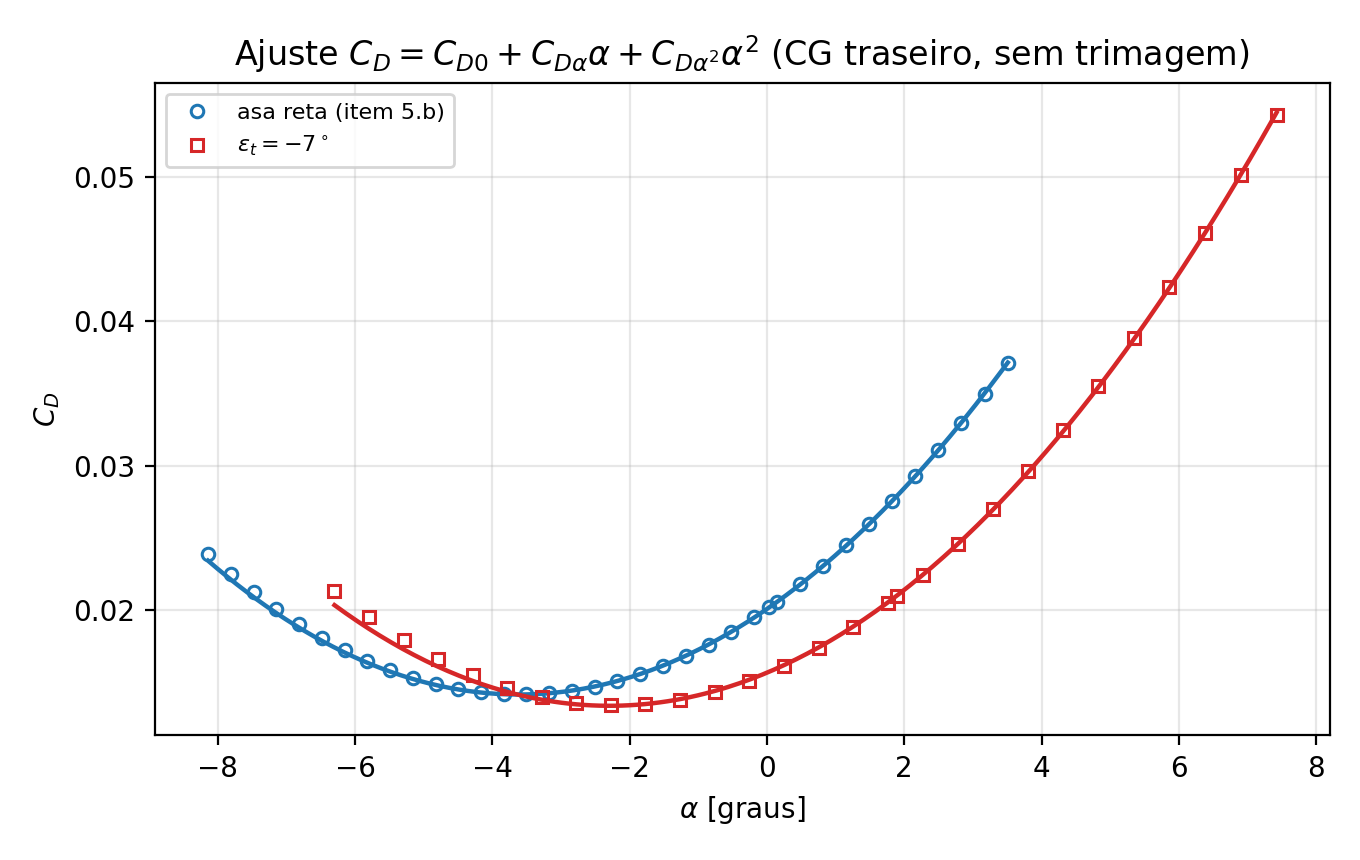
\includegraphics[width=0.78\textwidth]{resultados_s3/ajuste_polar_quadratica.png}
\caption{Ajuste quadrático $C_D(\alpha)$ da polar não trimada de CG traseiro.
Pontos do AVL e parábola da asa reta (item 5.b); em vermelho, o mesmo ajuste
com $\varepsilon_t = \esTwist^\circ$.}
\label{fig:ajuste-polar-quadratica}
\end{figure}

\begin{table}[H]
\centering
\caption{Ajuste quadrático para a polar de arrasto (asa reta, item 5.b).}
\label{tab:ajuste-quadratico}
\begin{tabular}{llc}
\toprule
Parametro & Descricao & Valor \\
\midrule
$C_{D0}$ & Termo constante da polar de arrasto & $0.02010$ \\
$C_{D\alpha}$ & Termo linear da polar [1/rad] & $0.18763$ \\
$C_{D\alpha^2}$ & Termo quadratico da polar [1/rad$^2$] & $1.48578$ \\
\bottomrule
\end{tabular}

\end{table}

Como no item~5: $C_{D0} = \esCD0Fit$ \textbf{não} é o arrasto parasita. Com
$i_w = \esIw^\circ$, $\alpha = 0$ já é quase o ponto de projeto, e o termo
constante carrega induzido e onda. Os três coeficientes só fazem sentido juntos.

\subsection{Derivadas no ponto de projeto}
\label{sec:estab-derivadas-projeto}

A Tab.~\ref{tab:derivadas-projeto} é a tabela do enunciado preenchida para a
\textbf{asa reta}, no $C_L = \esCL$ com $i_t = \esItReta^\circ$ e $\delta_e = 0$.
O AVL linearizou em $\alpha = \esAlpha^\circ$ de fuselagem. Esse é o jogo de
números que deve ir para o MVFO, coerente com os itens 3 e 5.

\begin{table}[H]
\centering
\caption{Informações e derivadas de estabilidade e controle no ponto de
projeto (asa reta, CG traseiro).}
\label{tab:derivadas-projeto}
\scriptsize
\begin{tabular}{llc}
\toprule
Parametro & Descricao & Valor \\
\midrule
$S_{\mathrm{ref}}$ & Area de referencia [m$^2$] & $382.9341$ \\
$c_{\mathrm{ref}}$ & Corda de referencia [m] & $6.9041$ \\
$b_{\mathrm{ref}}$ & Envergadura de referencia [m] & $63.6815$ \\
$m$ & Massa da aeronave [kg] & $221898$ \\
$I_{xx}$ & Momento de inercia [kg$\cdot$m$^2$] & $1.479e+07$ \\
$I_{yy}$ & Momento de inercia [kg$\cdot$m$^2$] & $4.632e+07$ \\
$I_{zz}$ & Momento de inercia [kg$\cdot$m$^2$] & $5.928e+07$ \\
$I_{xz}$ & Momento de inercia [kg$\cdot$m$^2$] & $1.130e+06$ \\
$i_p$ & Incidencia do motor [$^\circ$] & $0.0$ \\
$x_p$ & Posicao longitudinal do motor [m] & $19.416$ \\
$z_p$ & Posicao vertical do motor [m] (sinal invertido) & $2.985$ \\
$T_{\max}$ & Tracao maxima [N] & $777193$ \\
$V$ & Velocidade de voo [m/s] & $252.10$ \\
$h$ & Altitude de voo [m] & $10668$ \\
$C_{L0}$ & $C_L$ para $\alpha=0$ & $0.48779$ \\
$C_{L\alpha}$ & $\partial C_L/\partial\alpha$ [1/rad] & $6.75946$ \\
$C_{Lq}$ & $\partial C_L/\partial q$ [1/rad] & $7.71830$ \\
$C_{Li_t}$ & $\partial C_L/\partial i_t$ [1/rad] (mult.\ $180/\pi$) & $0.64148$ \\
$C_{L\delta_e}$ & $\partial C_L/\partial\delta_e$ [1/rad] (mult.\ $180/\pi$) & $0.40267$ \\
$C_{D0}$ & $C_D$ para $\alpha=0$ (ajuste 5.b) & $0.02010$ \\
$C_{D\alpha}$ & Termo linear da polar [1/rad] & $0.18763$ \\
$C_{D\alpha^2}$ & Termo quadratico da polar [1/rad$^2$] & $1.48578$ \\
$C_{Dq}$ & $\partial C_D/\partial q$ [1/rad] & $0.74085$ \\
$C_{Di_t}$ & $\partial C_D/\partial i_t$ [1/rad] (mult.\ $180/\pi$) & $0.01685$ \\
$C_{D\delta_e}$ & $\partial C_D/\partial\delta_e$ [1/rad] (mult.\ $180/\pi$) & $-0.00335$ \\
$C_{M0}$ & $C_M$ para $\alpha=0$ & $-0.10560$ \\
$C_{M\alpha}$ & $\partial C_M/\partial\alpha$ [1/rad] & $-0.21453$ \\
$C_{Mq}$ & $\partial C_M/\partial q$ [1/rad] & $-40.64451$ \\
$C_{Mi_t}$ & $\partial C_M/\partial i_t$ [1/rad] (mult.\ $180/\pi$) & $-3.09340$ \\
$C_{M\delta_e}$ & $\partial C_M/\partial\delta_e$ [1/rad] (mult.\ $180/\pi$) & $-2.00736$ \\
$C_{Y\beta}$ & $\partial C_Y/\partial\beta$ [1/rad] (sinal invertido) & $0.56290$ \\
$C_{Yp}$ & $\partial C_Y/\partial p$ [1/rad] (sinal invertido) & $-0.02170$ \\
$C_{Yr}$ & $\partial C_Y/\partial r$ [1/rad] (sinal invertido) & $0.16990$ \\
$C_{Y\delta_r}$ & $\partial C_Y/\partial\delta_r$ [1/rad] (mult.\ $180/\pi$) & $-0.15911$ \\
$C_{\ell\beta}$ & $\partial C_\ell/\partial\beta$ [1/rad] & $-0.19917$ \\
$C_{\ell p}$ & $\partial C_\ell/\partial p$ [1/rad] & $-0.55255$ \\
$C_{\ell r}$ & $\partial C_\ell/\partial r$ [1/rad] & $0.17647$ \\
$C_{\ell\delta_a}$ & $\partial C_\ell/\partial\delta_a$ [1/rad] (inv., $180/\pi$) & $-0.18782$ \\
$C_{\ell\delta_r}$ & $\partial C_\ell/\partial\delta_r$ [1/rad] (inv., $180/\pi$) & $0.01856$ \\
$C_{n\beta}$ & $\partial C_n/\partial\beta$ [1/rad] & $-0.13257$ \\
$C_{np}$ & $\partial C_n/\partial p$ [1/rad] & $-0.03516$ \\
$C_{nr}$ & $\partial C_n/\partial r$ [1/rad] & $-0.15627$ \\
$C_{n\delta_a}$ & $\partial C_n/\partial\delta_a$ [1/rad] (inv., $180/\pi$) & $0.01324$ \\
$C_{n\delta_r}$ & $\partial C_n/\partial\delta_r$ [1/rad] (inv., $180/\pi$) & $-0.08789$ \\
\bottomrule
\end{tabular}

\end{table}

\subsection{Efeito da torção geométrica nas derivadas}
\label{sec:estab-washout}

A Seção~\ref{sec:washout} adotou $\varepsilon_t = -7^\circ$ e recalculou
o $i_t$ do CG traseiro para $+0{,}330^\circ$. Esta subseção --- no mesmo
espírito da Seção~\ref{sec:washout-polar} --- repete as duas sessões do AVL
no \code{aft\_washout.avl}, com esse $i_t$, e confronta \textbf{todas} as
grandezas aerodinâmicas da Tab.~\ref{tab:derivadas-projeto} com a asa reta.
Massa, inércias, $x_p$, $z_p$, $i_p$ e $T_{\max}$ são os mesmos por
construção e não entram na comparação. A Tab.~\ref{tab:estab-washout} lista
o restante, com diferença absoluta e percentual; ``troca sinal'' marca os
casos em que o percentual não tem sentido.

Duas coisas mudam ao mesmo tempo e não se separam nesta comparação: a
\textbf{geometria} da asa e o \textbf{ponto de linearização} ($\alpha$ de
$0{,}036^\circ$ para $1{,}898^\circ$, $i_t$ de $-1{,}959^\circ$ para
$+0{,}330^\circ$). Os dois efeitos estão em todas as colunas.

\begin{table}[H]
\centering
\caption{Comparação completa das grandezas aerodinâmicas da Seção~3, CG
traseiro: asa reta (\code{aft.avl}) versus $\varepsilon_t = -7^\circ$
(\code{aft\_washout.avl}). A tabela oficial do MVFO continua sendo a da asa
reta.}
\label{tab:estab-washout}
\scriptsize
\begin{tabular}{lrrrl}
\toprule
Parametro & Asa reta & $\varepsilon_t=-7^\circ$ & $\Delta$ & $\Delta$ [\%] \\
\midrule
$i_t$ de equilibrio [$^\circ$] & $-1.95893$ & $0.33027$ & $+2.28920$ & troca sinal \\
$\alpha$ no ponto [$^\circ$] & $0.03634$ & $1.89832$ & $+1.86198$ & --- \\
$C_D$ no ponto de projeto & $0.02023$ & $0.02102$ & $+0.00079$ & $+3.91$ \\
$C_{L0}$ ($\alpha=0$, $i_t=0$) & $0.48779$ & $0.24275$ & $-0.24504$ & $-50.23$ \\
$C_{M0}$ ($\alpha=0$, $i_t=0$) & $-0.10560$ & $0.02450$ & $+0.13010$ & troca sinal \\
$C_D$ em $\alpha=0$, $i_t=0$ & $0.02033$ & $0.01553$ & $-0.00480$ & $-23.61$ \\
$C_{L\alpha}$ & $6.75946$ & $6.73275$ & $-0.02671$ & $-0.40$ \\
$C_{Lq}$ & $7.71830$ & $7.55218$ & $-0.16612$ & $-2.15$ \\
$C_{Li_t}$ & $0.64148$ & $0.64005$ & $-0.00143$ & $-0.22$ \\
$C_{L\delta_e}$ & $0.40267$ & $0.40050$ & $-0.00218$ & $-0.54$ \\
$C_{D0}$ (ajuste 5.b) & $0.02010$ & $0.01569$ & $-0.00441$ & $-21.95$ \\
$C_{D\alpha}$ (ajuste 5.b) & $0.18763$ & $0.11440$ & $-0.07324$ & $-39.03$ \\
$C_{D\alpha^2}$ (ajuste 5.b) & $1.48578$ & $1.42705$ & $-0.05873$ & $-3.95$ \\
$C_{Dq}$ & $0.74085$ & $0.63715$ & $-0.10370$ & $-14.00$ \\
$C_{Di_t}$ & $0.01685$ & $0.03514$ & $+0.01829$ & $+108.56$ \\
$C_{D\delta_e}$ & $-0.00335$ & $0.01815$ & $+0.02150$ & troca sinal \\
$C_{M\alpha}$ & $-0.21453$ & $-0.17965$ & $+0.03488$ & $-16.26$ \\
$C_{Mq}$ & $-40.64451$ & $-40.36494$ & $+0.27957$ & $-0.69$ \\
$C_{Mi_t}$ & $-3.09340$ & $-3.09157$ & $+0.00183$ & $-0.06$ \\
$C_{M\delta_e}$ & $-2.00736$ & $-1.99292$ & $+0.01444$ & $-0.72$ \\
$C_{Y\beta}$ & $0.56290$ & $0.55660$ & $-0.00630$ & $-1.12$ \\
$C_{Yp}$ & $-0.02170$ & $-0.03995$ & $-0.01825$ & $+84.11$ \\
$C_{Yr}$ & $0.16990$ & $0.18401$ & $+0.01411$ & $+8.30$ \\
$C_{Y\delta_r}$ & $-0.15911$ & $-0.15848$ & $+0.00063$ & $-0.40$ \\
$C_{\ell\beta}$ & $-0.19917$ & $-0.15903$ & $+0.04014$ & $-20.15$ \\
$C_{\ell p}$ & $-0.55255$ & $-0.55704$ & $-0.00449$ & $+0.81$ \\
$C_{\ell r}$ & $0.17647$ & $0.10232$ & $-0.07415$ & $-42.02$ \\
$C_{\ell\delta_a}$ & $-0.18782$ & $-0.18816$ & $-0.00034$ & $+0.18$ \\
$C_{\ell\delta_r}$ & $0.01856$ & $0.01839$ & $-0.00017$ & $-0.93$ \\
$C_{n\beta}$ & $-0.13257$ & $-0.12782$ & $+0.00476$ & $-3.59$ \\
$C_{np}$ & $-0.03516$ & $-0.04525$ & $-0.01008$ & $+28.67$ \\
$C_{nr}$ & $-0.15627$ & $-0.15642$ & $-0.00015$ & $+0.09$ \\
$C_{n\delta_a}$ & $0.01324$ & $-0.00561$ & $-0.01885$ & troca sinal \\
$C_{n\delta_r}$ & $-0.08789$ & $-0.08743$ & $+0.00046$ & $-0.52$ \\
$X_{np}$ [m] & $30.12918$ & $30.09429$ & $-0.03489$ & $-0.12$ \\
SM AVL [\%] & $3.17375$ & $2.66832$ & $-0.50542$ & $-15.93$ \\
\bottomrule
\end{tabular}

\end{table}

\paragraph{Equilíbrio e termos de $\alpha=0$.}
$C_{L0}$ cai de $0{,}48779$ para $0{,}24275$ ($-50{,}2$\%): a ponta
descarregada produz menos sustentação a um dado $\alpha$. $C_{M0}$ passa de
$-0{,}10560$ para $+0{,}02450$ e \textbf{troca de sinal} --- o momento da
asa fica cabrador, e é por isso que o $i_t$ de equilíbrio cruza zero. O
$C_D$ em $\alpha=0$, $i_t=0$ cai de $0{,}02033$ para $0{,}01553$, porque
esse ponto agora corresponde a um $C_L$ bem menor. No ponto de projeto o
$C_D$ sobe de $0{,}02023$ para $0{,}02102$ ($+3{,}9$\%), o mesmo já visto
na polar do item~5 no CG traseiro.

\paragraph{Longitudinais de $C_L$ e $C_M$.}
$C_{L\alpha}$ mal se mexeu ($6{,}759$ para $6{,}733$, $-0{,}4$\%): a área e
o enflechamento são os mesmos. $C_{Lq}$ cai de $7{,}718$ para $7{,}552$
($-2{,}2$\%), um pouco menos de sustentação por taxa de arfagem com a ponta
mais leve. $C_{M\alpha}$ é a derivada longitudinal que mais muda,
$-0{,}215$ para $-0{,}180$ ($-16{,}3$\%): o avião continua estável, mas a
margem encolhe. $C_{Mq}$ passa de $-40{,}64$ para $-40{,}36$ (menos de
$1$\%). O $X_{np}$ recua de $30{,}129$~m para $30{,}094$~m e a margem
estática AVL de $3{,}2$\% para $2{,}7$\%.

\paragraph{Comandos de empenagem.}
A EH não foi torcida. $C_{Li_t}$ vai de $0{,}6415$ para $0{,}6401$ e
$C_{Mi_t}$ de $-3{,}0934$ para $-3{,}0916$; $C_{L\delta_e}$ de $0{,}4027$
para $0{,}4005$ e $C_{M\delta_e}$ de $-2{,}0074$ para $-1{,}9929$. Tudo
abaixo de $1$\%. O que muda de verdade no canal de arfagem é o $i_t$ em que
se lineariza, não a autoridade da cauda.

\paragraph{Arrasto: derivadas e ajuste 5.b.}
$C_{Dq}$ cai de $0{,}741$ para $0{,}637$ ($-14{,}0$\%). $C_{Di_t}$ sobe de
$0{,}0169$ para $0{,}0351$ ($+108{,}6$\%): com a EH sustentando ($i_t>0$) o
mesmo $\Delta i_t$ custa mais arrasto induzido. $C_{D\delta_e}$ troca de
sinal, $-0{,}0034$ para $+0{,}0181$. O ajuste quadrático da polar 5.b ---
refeito na asa torcida --- passa de
$(C_{D0},C_{D\alpha},C_{D\alpha^2})=(0{,}02010,\,0{,}18763,\,1{,}48578)$
para $(0{,}01569,\,0{,}11440,\,1{,}42705)$. A queda do termo constante não
é ``menos arrasto'': $\alpha=0$ agora é um $C_L$ menor, e a origem da
parábola anda com ele.

\paragraph{Látero-direcionais estáticas.}
$C_{Y\beta}$ vai de $0{,}563$ para $0{,}557$ ($-1{,}1$\%). $C_{n\beta}$ de
$-0{,}133$ para $-0{,}128$ ($-3{,}6$\%): a deriva não mudou.
$C_{\ell\beta}$ cai de $-0{,}199$ para $-0{,}159$ ($-20{,}2$\%):
descarregar a ponta de uma asa enflechada reduz o diedro efetivo, e isso
aparece no rolamento por derrapagem.

\paragraph{Amortecimentos e acoplamentos laterais.}
$C_{\ell p}$ quase não se mexe ($-0{,}553$ para $-0{,}557$). $C_{nr}$ idem
($-0{,}156$ nos dois). O que muda é o acoplamento: $C_{\ell r}$ cai de
$0{,}176$ para $0{,}102$ ($-42{,}0$\%); $C_{Yp}$ de $-0{,}022$ para
$-0{,}040$ ($+84{,}1$\%); $C_{Yr}$ de $0{,}170$ para $0{,}184$
($+8{,}3$\%); $C_{np}$ de $-0{,}035$ para $-0{,}045$ ($+28{,}7$\%). Parte
disso é ponta mais leve, parte é o $\alpha$ de linearização $\sim 2^\circ$
em vez de $\sim 0^\circ$. Não dá para atribuir o $\Delta$ só à torção.

\paragraph{Aileron e leme.}
$C_{\ell\delta_a}$ ($-0{,}1878$ para $-0{,}1882$), $C_{\ell\delta_r}$
($0{,}0186$ para $0{,}0184$), $C_{Y\delta_r}$ ($-0{,}1591$ para
$-0{,}1585$) e $C_{n\delta_r}$ ($-0{,}0879$ para $-0{,}0874$) ficam abaixo
de $1$\%. A exceção é $C_{n\delta_a}$, que \textbf{troca de sinal}:
$+0{,}0132$ para $-0{,}0056$. O yaw adverso do aileron inverte na asa
torcida, de novo com a ressalva de que o AVL linearizou noutro $\alpha$.

\subsection{Discussão}

$C_{L\alpha} = \esCLa$~rad$^{-1}$ é o sinal e a ordem certos para um transporte
de $\Lambda \approx 35^\circ$ e $AR \approx 10{,}6$. $C_{M\alpha} = \esCma$ é
negativo: o avião é estaticamente estável em arfagem no CG traseiro. A margem
que o AVL enxerga,
$(X_{np}-X_{cg})/\bar{c} = \esSM$\%, é menor que os $10$\% do
\code{designTool} --- o mesmo viés já visto no item~3, e o motivo de se
trabalhar com o $X_{\mathrm{ref}}$ do CG e não com o NP empírico.

$C_{\ell\beta} = \esClb$ negativo é o efeito diedro (incluindo o diedro
efetivo da asa enflechada). $C_{\ell p} = \esClp$ e $C_{nr} = \esCnr$ são os
amortecimentos de rolamento e de guinada, ambos com o sinal estabilizante
esperado. $C_{n\beta} = \esCnb$ sai \emph{negativo} do AVL. Na convenção
``$X$ para frente, $Z$ para baixo'' do próprio \code{st} isso deveria ser
positivo (weathercock). O número foi transcrito sem inversão extra --- o
roteiro não pede para virar $C_{n\beta}$ --- e deve ser lido com essa ressalva
na hora de montar o MVFO: se o modo espiral ou o rolamento holandês
aparecerem instáveis, o primeiro suspeito é o sinal de $C_{n\beta}$, não a
planta da deriva.

Os comandos têm o sinal que o MVFO espera depois das inversões: profundor
$C_{L\delta_e} = \esCLd4 > 0$ e $C_{M\delta_e} = \esCmd4 < 0$ (cabra o nariz
quando $\delta_e > 0$ no AVL); $i_t$ entra com
$C_{Li_t} = \esCLg1$ e $C_{Mi_t} = \esCmg1$, o mesmo papel do profundor em
escala maior. Aileron e leme já estão com o sinal do MVFO na
Tab.~\ref{tab:derivadas-projeto}.

O motor entra só como ponto de força ($x_p = \esXp$~m, $z_p = \esZp$~m,
$i_p = 0$). O AVL não modela jato nem efeito de esteira na EH; as derivadas
aerodinâmicas desta seção são de avião \emph{planador} no $C_L$ de cruzeiro.
O $T_{\max}$ da Tab.~\ref{tab:dados-gerais-estabilidade} é para o MVFO
montar o termo de empuxo, não para o AVL.

A torção de $-7^\circ$ \textbf{não} foi adotada na tabela oficial do
MVFO. A Tab.~\ref{tab:estab-washout} é o inventário completo do que mudaria
se ela o fosse: equilíbrio ($C_{L0}$, $C_{M0}$, $i_t$, $\alpha$),
$C_{M\alpha}$ e margem estática, o bloco de arrasto ($C_{Dq}$, $C_{Di_t}$,
$C_{D\delta_e}$ e o ajuste 5.b), o diedro efetivo $C_{\ell\beta}$, os
acoplamentos $C_{\ell r}$, $C_{Yp}$, $C_{Yr}$, $C_{np}$ e o sinal de
$C_{n\delta_a}$. Até lá, o arquivo que o MVFO deve ler é a
Tab.~\ref{tab:derivadas-projeto}.
